In Figure \ref{fig:CfrAverage}, the average correlation distributions from the published analysis in p-Pb 2013 sample (black points) and the new p-Pb 2016 sample (red points), both at 5 TeV, are compared. As it's evident, the statistical and systematic uncertainties are largely reduced in the new data sample. The feature of the correlation distributions are the same in both systems, and an overall compatibility of the shapes is observed. 

\begin{figure}[!htbp]
\centering
%Marianna
\centering
{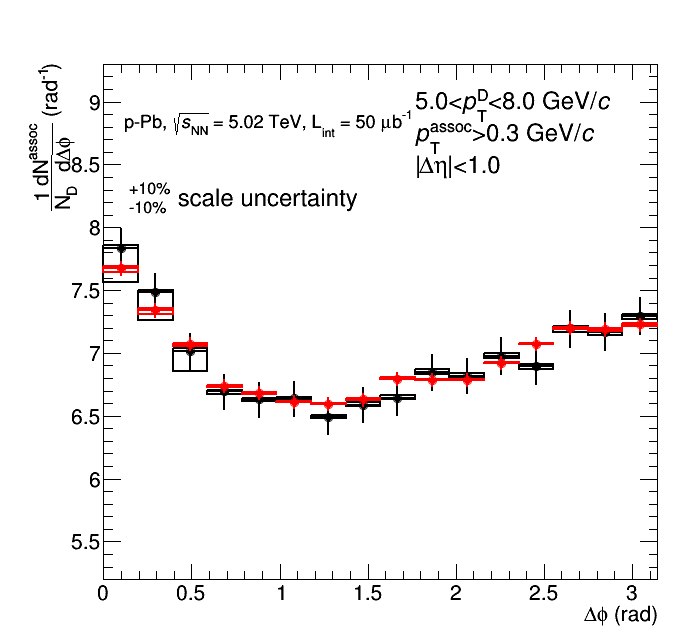
\includegraphics[width=0.47\linewidth]{figures/Cfr2013vs2016/Average_Cfr_2013_2016_Pt5to8_Thr03to99.png}}
{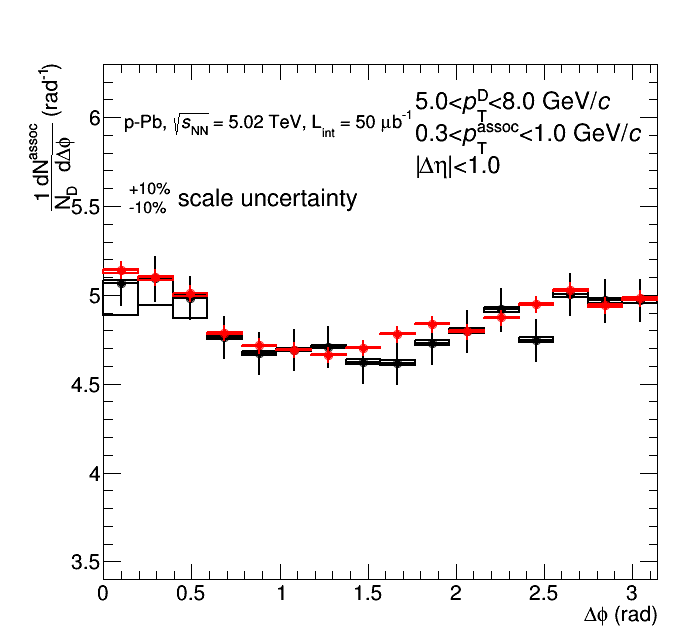
\includegraphics[width=0.47\linewidth]{figures/Cfr2013vs2016/Average_Cfr_2013_2016_Pt5to8_Thr03to1.png}}
{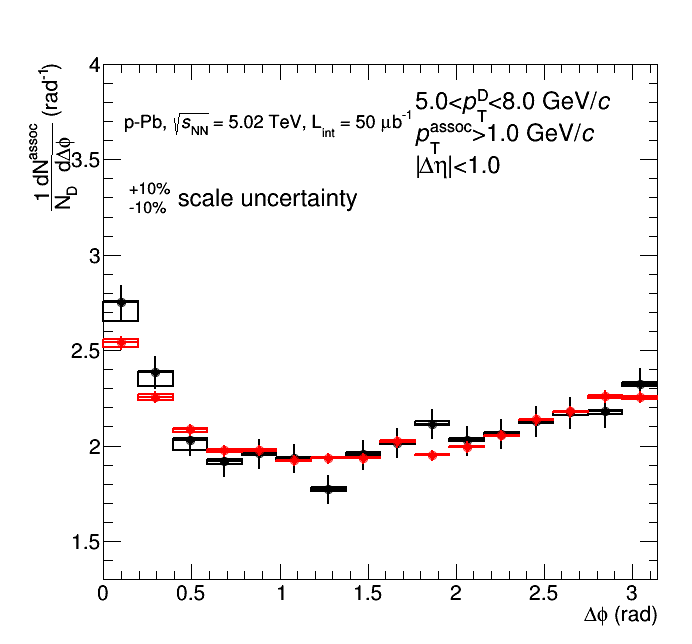
\includegraphics[width=0.47\linewidth]{figures/Cfr2013vs2016/Average_Cfr_2013_2016_Pt5to8_Thr1to99.png}}
{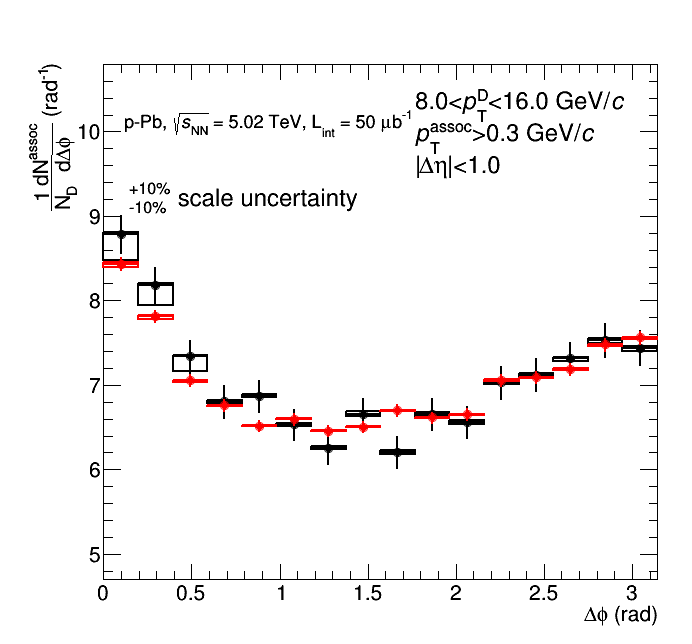
\includegraphics[width=0.47\linewidth]{figures/Cfr2013vs2016/Average_Cfr_2013_2016_Pt8to16_Thr03to99.png}}
{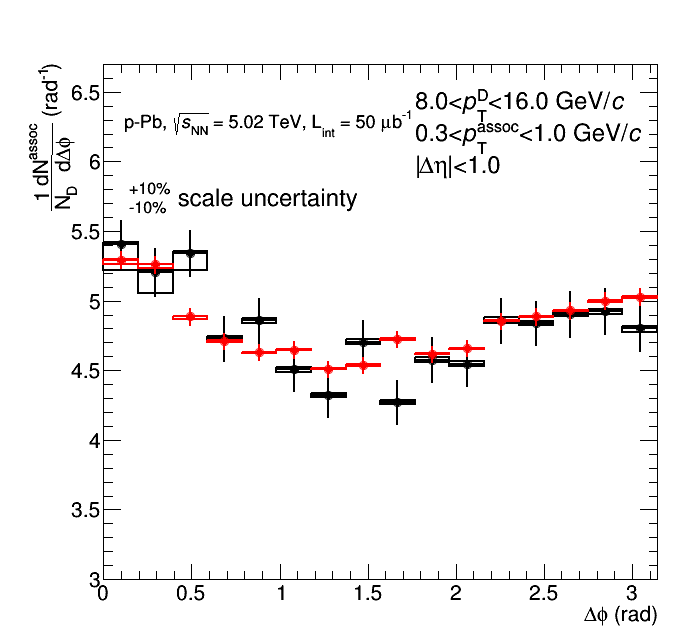
\includegraphics[width=0.47\linewidth]{figures/Cfr2013vs2016/Average_Cfr_2013_2016_Pt8to16_Thr03to1.png}}
{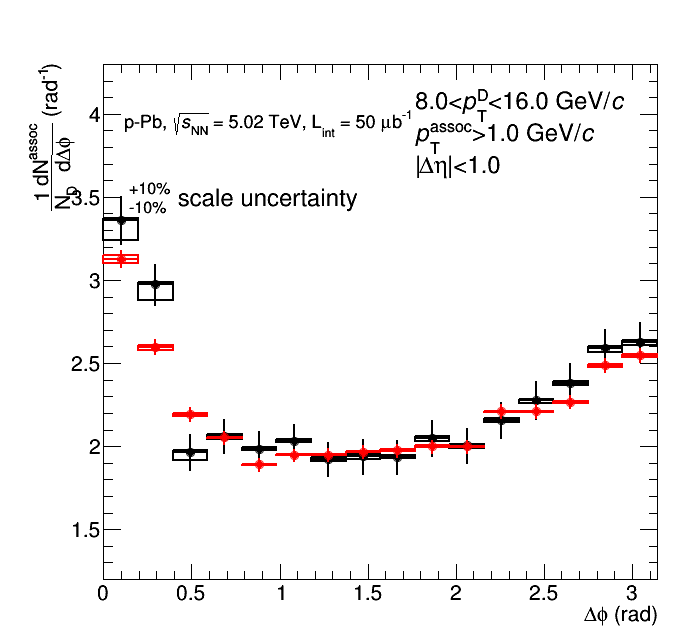
\includegraphics[width=0.47\linewidth]{figures/Cfr2013vs2016/Average_Cfr_2013_2016_Pt8to16_Thr1to99.png}}
\caption{Comparison of 2016 (red) and 2013 (black) results for azimuthal correlation distributions, for the common $\pt$ ranges.}
\label{fig:CfrAverage}
\end{figure}

Figure \ref{fig:CfrObs} shows the same comparison for the fit observables. Also in this case the uncertainties are largely reduced for the 2016 analysis. The near-side widths are on top of each other; for the near-side yields a slight decrease of the 2016 results is observed in some $\pt$ ranges with respect to 2013 results, though within the uncertainty, which were very large for the 2013 sample. The pedestal values are also fully compatible within the two samples. The sensitivity to away-side observables was very poor for 2013 results, hence a comparison with 2016 data is difficult, anyway, within the large uncertainties, also the away-side observables are compatible between the two datasets.

\begin{figure}[!htbp]
\centering
%Marianna
\centering
{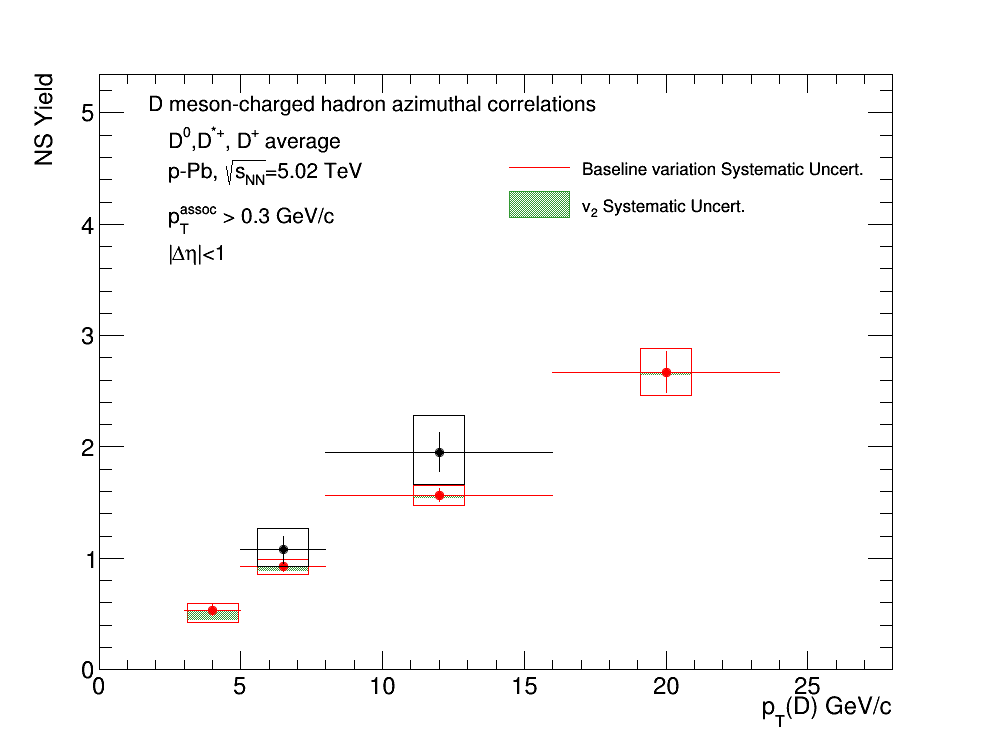
\includegraphics[width=0.31\linewidth]{figures/Cfr2013vs2016/NSYield_Cfr_2013_2016_Thr03to99.png}}
{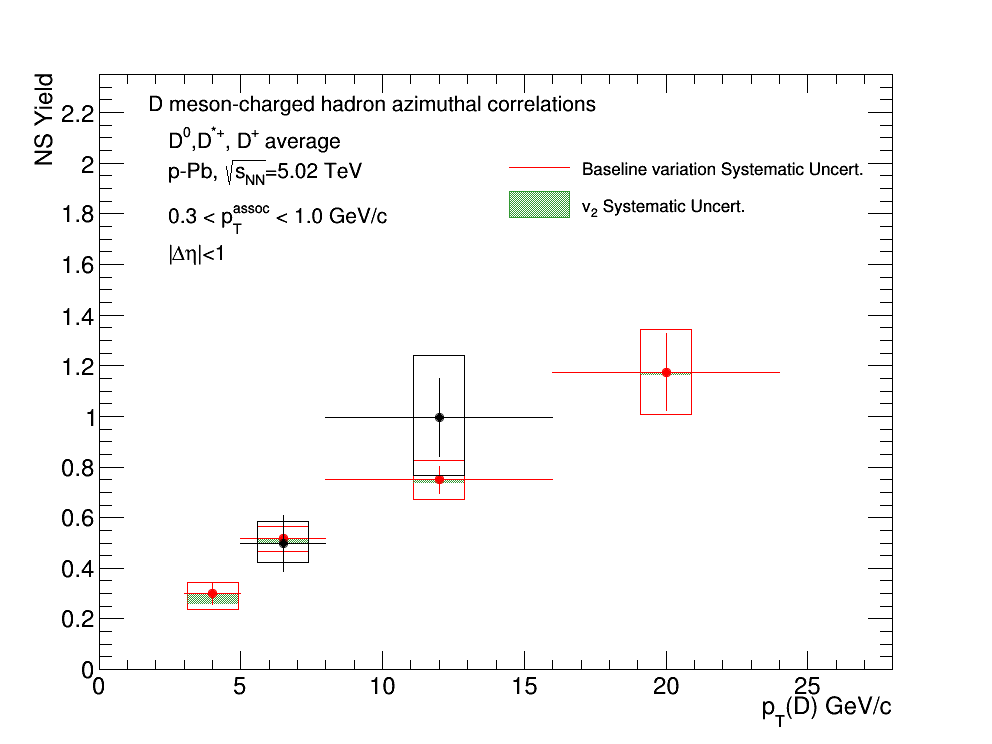
\includegraphics[width=0.31\linewidth]{figures/Cfr2013vs2016/NSYield_Cfr_2013_2016_Thr03to1.png}}
{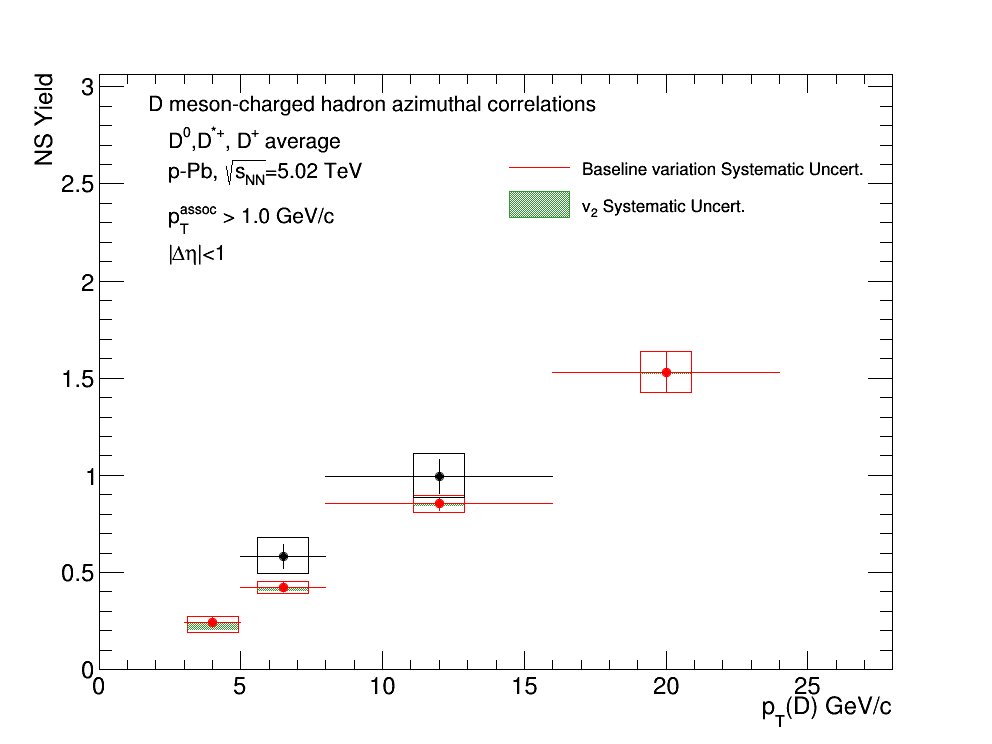
\includegraphics[width=0.31\linewidth]{figures/Cfr2013vs2016/NSYield_Cfr_2013_2016_Thr1to99.png}}
{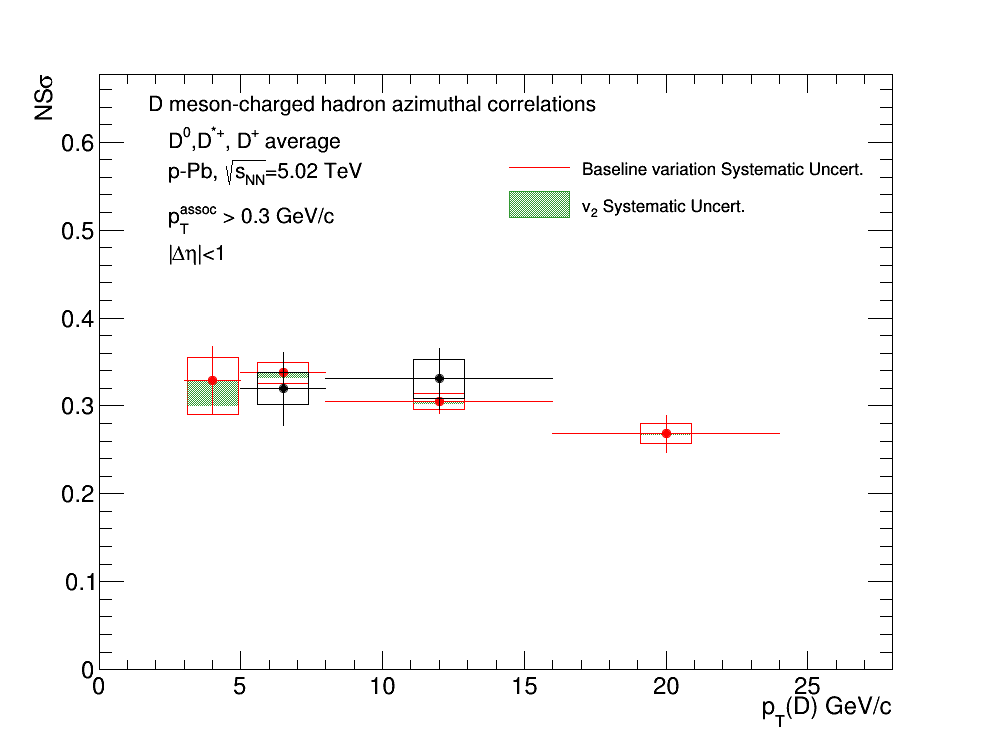
\includegraphics[width=0.31\linewidth]{figures/Cfr2013vs2016/NSsigma_Cfr_2013_2016_Thr03to99.png}}
{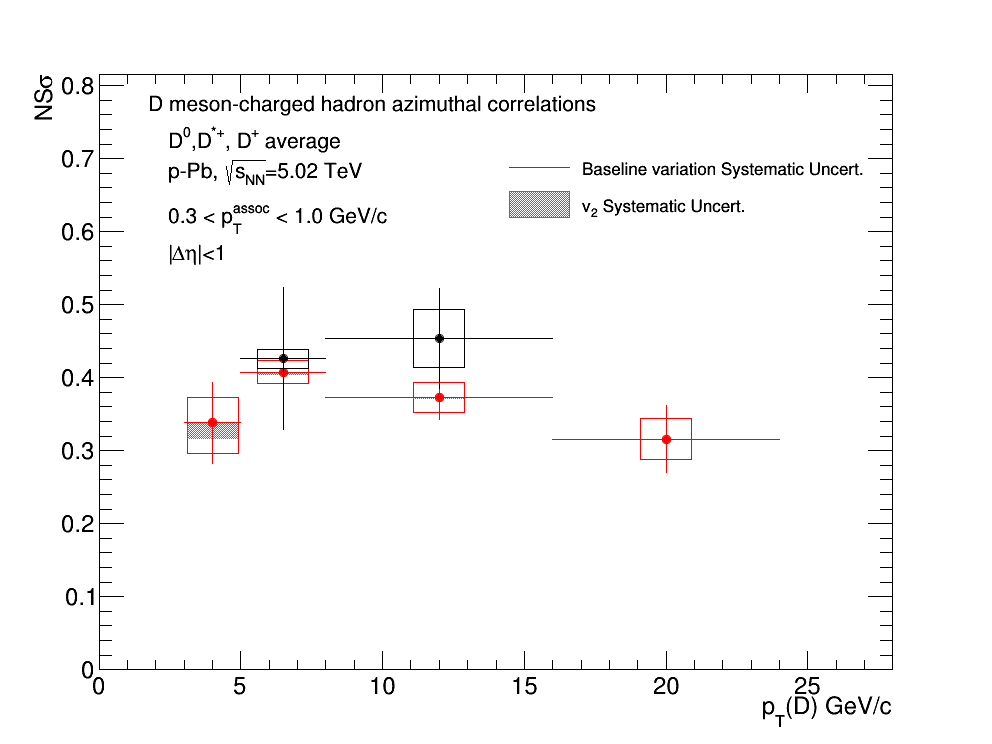
\includegraphics[width=0.31\linewidth]{figures/Cfr2013vs2016/NSsigma_Cfr_2013_2016_Thr03to1.png}}
{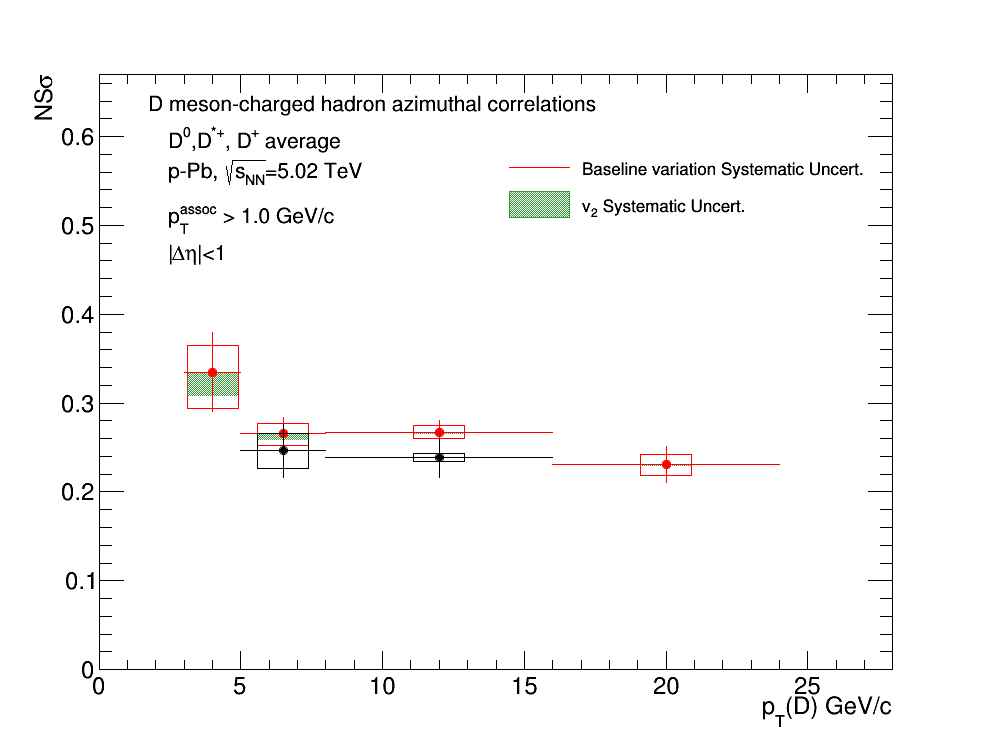
\includegraphics[width=0.31\linewidth]{figures/Cfr2013vs2016/NSsigma_Cfr_2013_2016_Thr1to99.png}}
{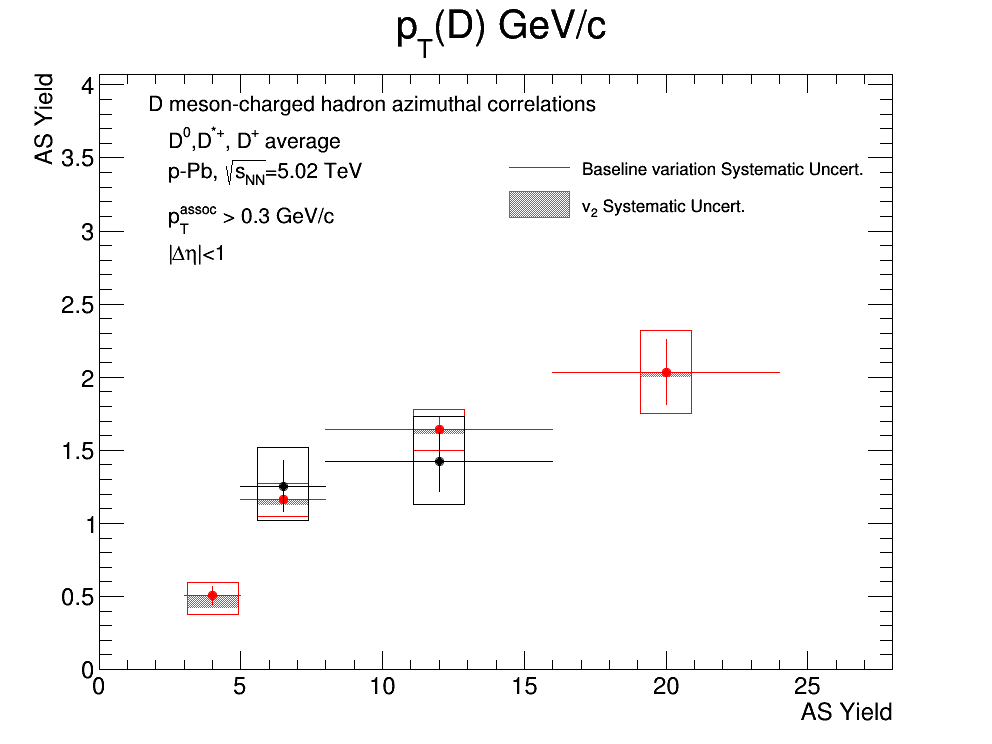
\includegraphics[width=0.31\linewidth]{figures/Cfr2013vs2016/ASYield_Cfr_2013_2016_Thr03to99.png}}
{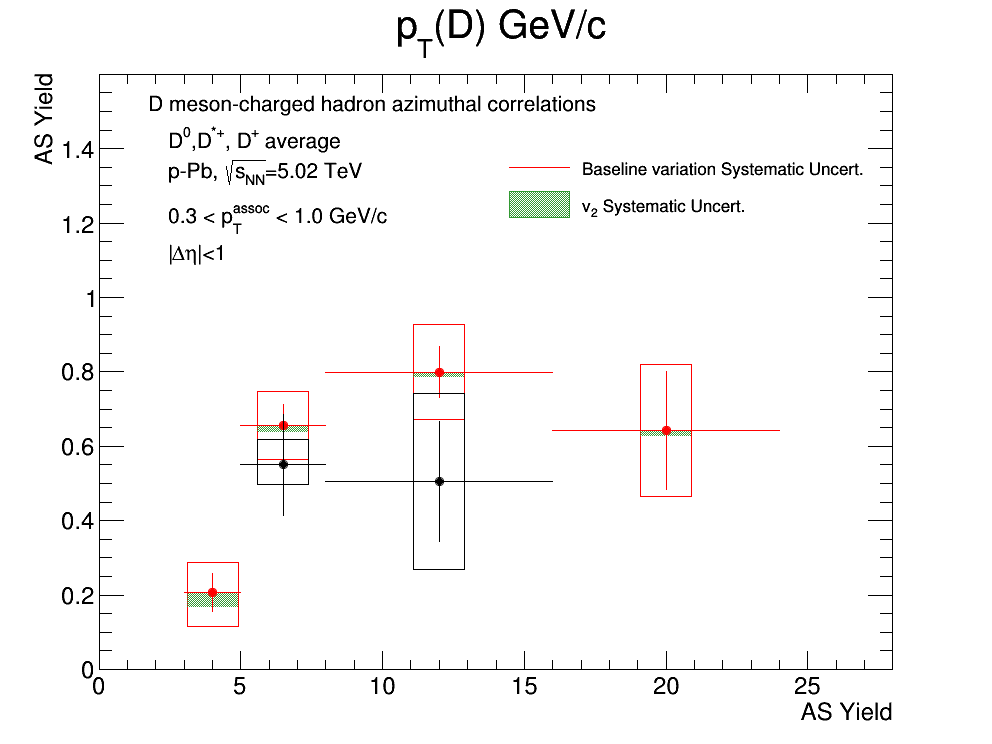
\includegraphics[width=0.31\linewidth]{figures/Cfr2013vs2016/ASYield_Cfr_2013_2016_Thr03to1.png}}
{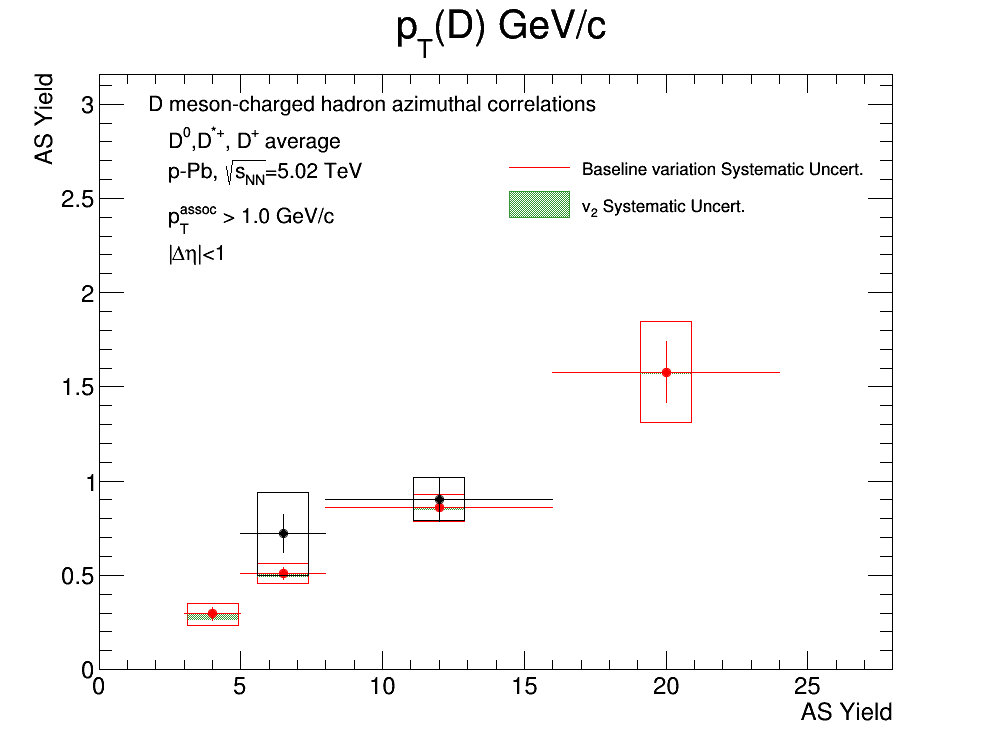
\includegraphics[width=0.31\linewidth]{figures/Cfr2013vs2016/ASYield_Cfr_2013_2016_Thr1to99.png}}
{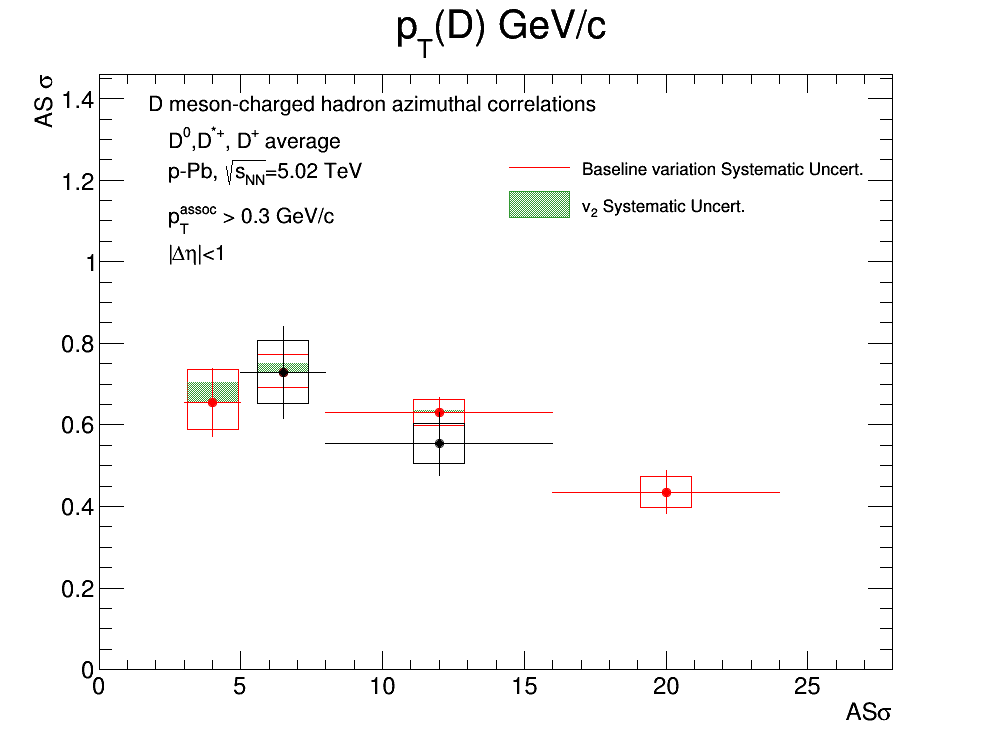
\includegraphics[width=0.31\linewidth]{figures/Cfr2013vs2016/ASsigma_Cfr_2013_2016_Thr03to99.png}}
{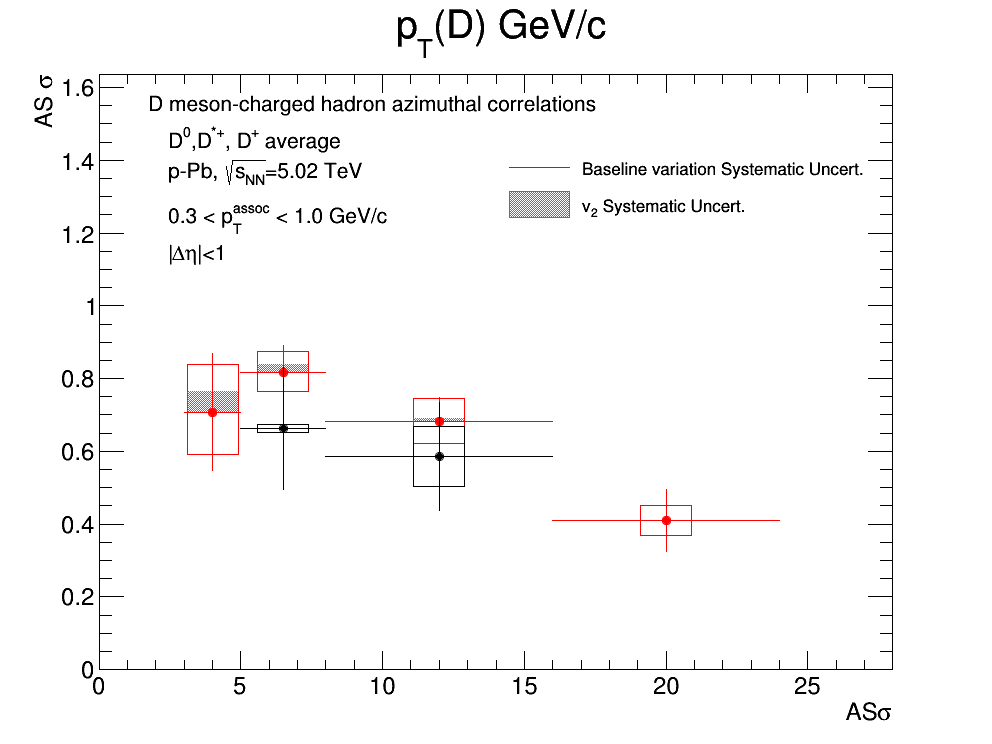
\includegraphics[width=0.31\linewidth]{figures/Cfr2013vs2016/ASsigma_Cfr_2013_2016_Thr03to1.png}}
{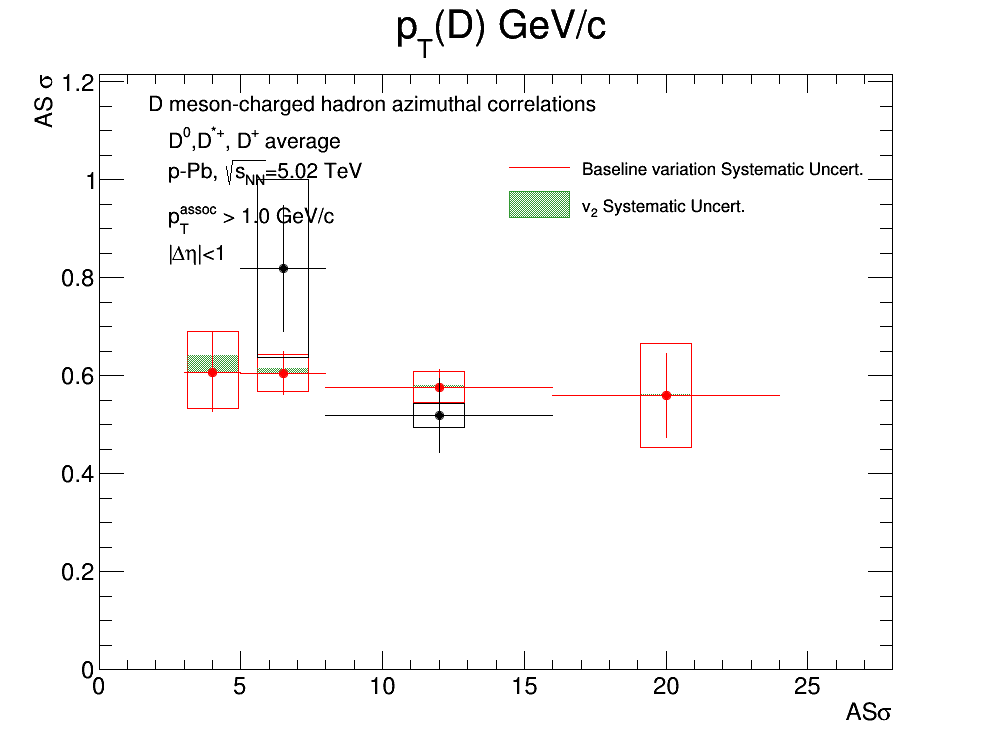
\includegraphics[width=0.31\linewidth]{figures/Cfr2013vs2016/ASsigma_Cfr_2013_2016_Thr1to99.png}}
{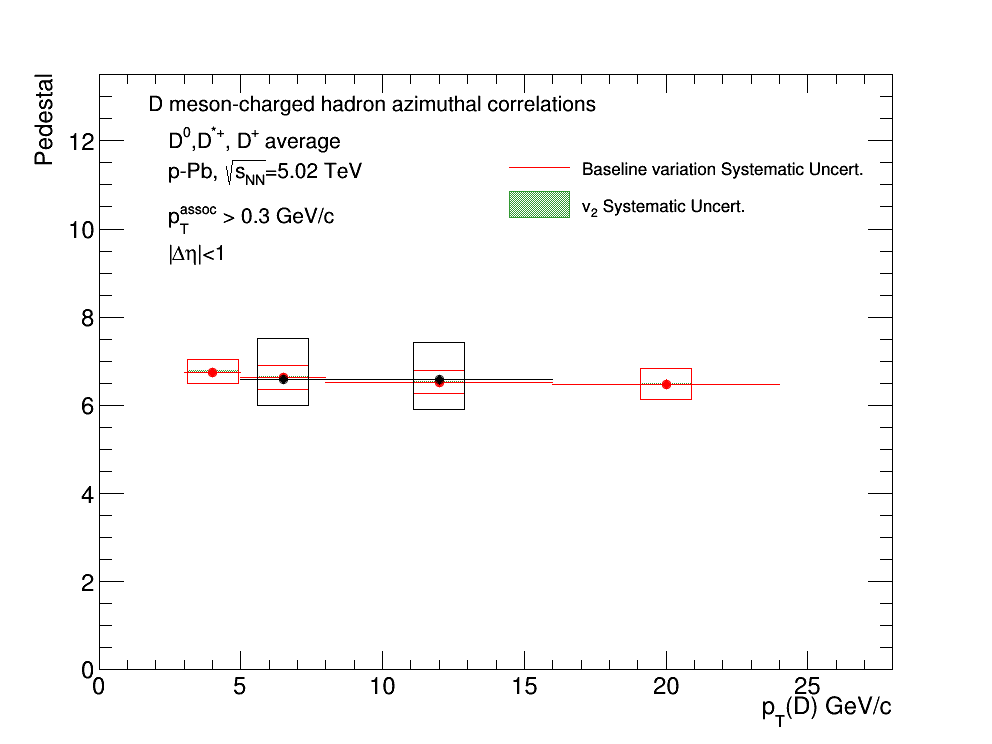
\includegraphics[width=0.31\linewidth]{figures/Cfr2013vs2016/Pedestal_Cfr_2013_2016_Thr03to99.png}}
{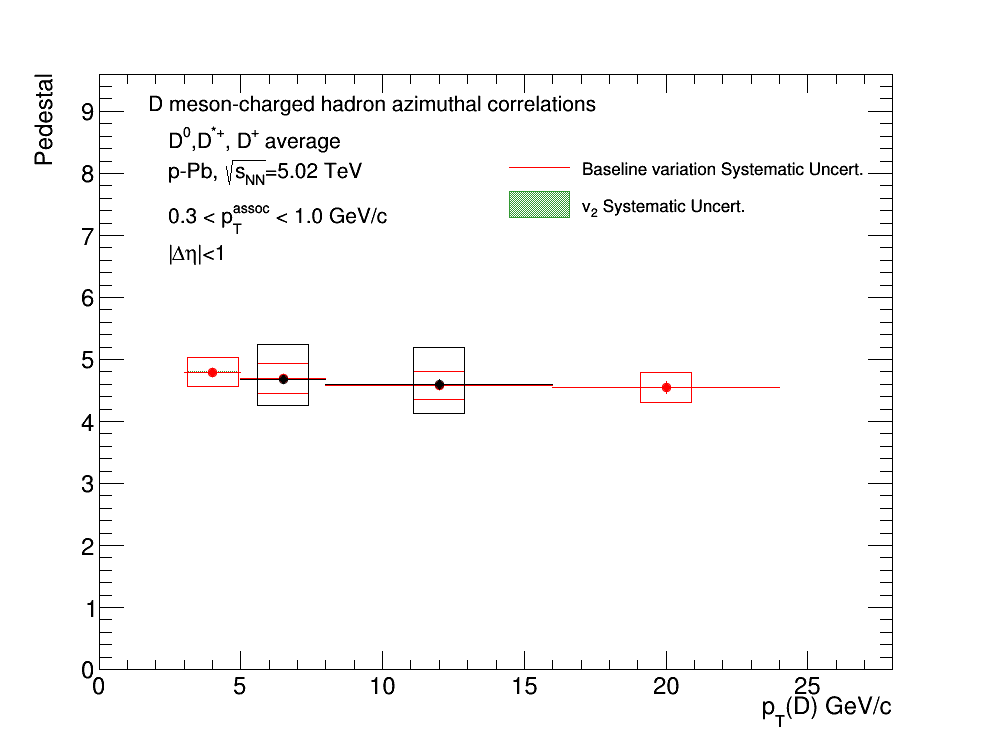
\includegraphics[width=0.31\linewidth]{figures/Cfr2013vs2016/Pedestal_Cfr_2013_2016_Thr03to1.png}}
{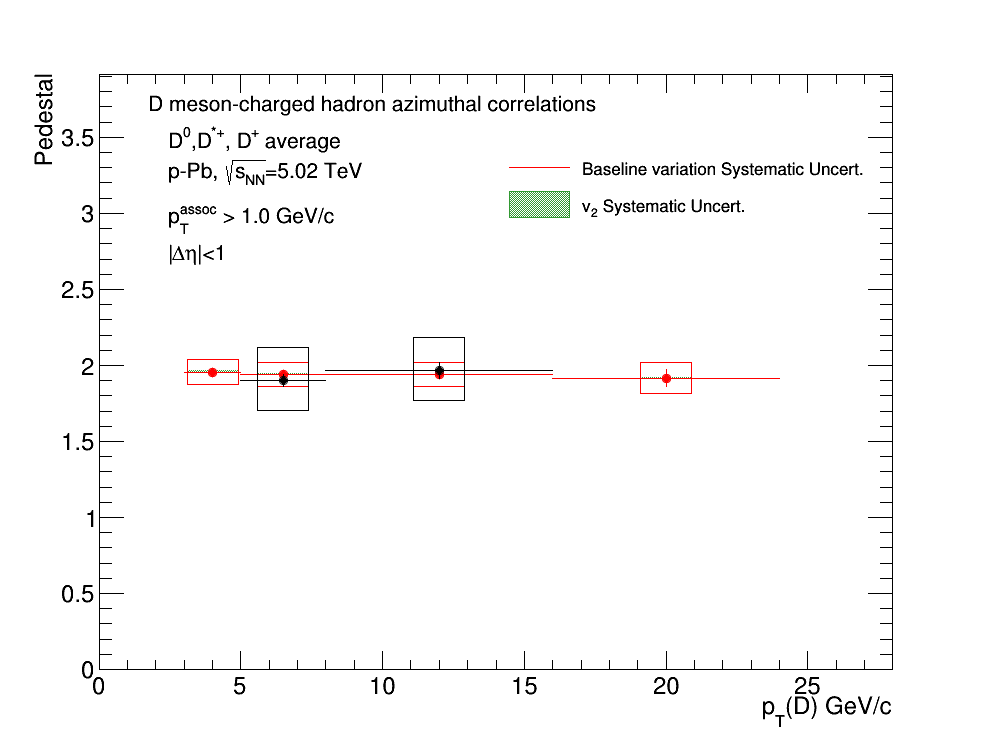
\includegraphics[width=0.31\linewidth]{figures/Cfr2013vs2016/Pedestal_Cfr_2013_2016_Thr1to99.png}}
\caption{Comparison of the average D-h azimuthal correlation properties between 2016 p-Pb (red) and 2013 p-Pb (black) data analysis, for the common $\pt$ ranges of D meson and associated particles.}
\label{fig:CfrObs}
\end{figure}
